\exercise

Given the set of strings $S$ = \{ {\tt abaa}, {\tt abca}, {\tt abma}, {\tt baa},
{\tt bbb} \}, build a Patricia trie and show the steps for the lexicographic
search of the strings $P_1$ = {\tt aaa}, $P_2$ = {\tt abb}.

\solution

\autoref{fig:patricia-trie} shows the graphical representation of the Patricia
trie built over $S$. The lexicographic searches are done as follows:
%
\begin{itemize}

  \item[$P_1$:] We first traverse the Patricia tree comparing the single
  characters on the edge of the trie, which produces a partial match on the
  first and third characters of $P_1$ ({\tt \underline{a}a\underline{a}}),
  pointing to the leaf node $S_0 = \text{\tt abaa}$. We compare $P_1$ and $S_0$
  and find the length of their shared prefix (which is also the longest common
  prefix among the strings indexed by the Patricia trie), which is $\ell = 1$.
  The Patricia trie is now traversed upward to find the mismatching position
  $S_0[\ell + 1]$, which is in the leftmost edge branching from the root node.
  Since $P_1[\ell + 1] < S_0[\ell + 1]$, $P_1$ lies at the left of that subtree,
  so $\forall s \in S.\ P_1 \prec s$.

  \item[$P_2$:] We first traverse the Patricia tree comparing the single
  characters on the edge of the trie, which produces a match only on the first
  character of $P_2$ ({\tt \underline{a}bb}). Since we do not have a match after
  the first edge, we choose any descendant leaf after the traversed node (say
  $S_1 = \text{\tt abca}$). We compare $P_2$ and $S_1$ and find the length of
  their shared prefix, which is $\ell = 2$. The Patricia trie is now traversed
  upward to find the mismatching position $S_1[\ell + 1]$, which is a branching
  character. Since $\text{\tt a} < P_2[\ell + 1] < \text{\tt c}$, $P_2$ lies
  between the rightmost string of the {\tt a}-branching subtree and the leftmost
  string of the {\tt c}-branching subtree, so $S_0 \prec P_2 \prec S_1$.

\end{itemize}
%
\begin{figure}[b]
  \centering
  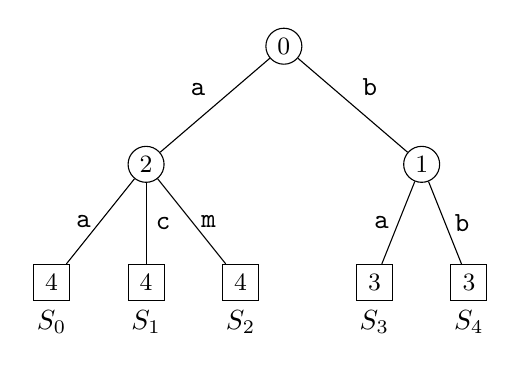
\begin{tikzpicture}[
    grow=down,
    inner/.style={draw, fill=white, inner sep=0, minimum size=13, circle},
    leaf/.style={draw, fill=white, inner sep=0, minimum size=13},
    level 1/.style={sibling distance = 3.5cm, level distance = 1.5cm},
    level 2/.style={sibling distance = 1.2cm, level distance = 1.5cm}
  ]
  \node[inner] {\small 0}
    child {
      node[inner] {\small 2}
      child {
          node[leaf, label=below:$S_0$] {\small 4}
          edge from parent[-] node[left] {\tt a}
      }
      child {
          node[leaf, label=below:$S_1$] {\small 4}
          edge from parent[-] node[right] {\tt c}
      }
      child {
          node[leaf, label=below:$S_2$] {\small 4}
          edge from parent[-] node[right] {\tt m}
      }
      edge from parent[-] node[above left] {\tt a}
    }
    child {
      node[inner] {\small 1}
      child {
          node[leaf, label=below:$S_3$] {\small 3}
          edge from parent[-] node[left] {\tt a}
      }
      child {
          node[leaf, label=below:$S_4$] {\small 3}
          edge from parent[-] node[right] {\tt b}
      }
      edge from parent[-] node[above right] {\tt b}
    };
  \end{tikzpicture}
  \caption{Graphical representation of the Patricia trie built over $S$.}
  \label{fig:patricia-trie}
\end{figure}
